\appendix
\pagenumbering{Roman}


\newappendix{Obsah elektronické přílohy}
\label{app:dirtree}
Zdrojové kódy firmware, software, návrh hardwarového řešení, elektronické
simulace, jakož i zdrojový kód této práce využívající systém pro počítačovou
sazbu \LaTeX{} jsou k práci přiloženy jako elektronická příloha. Ta je rozdělena
do několika adresářů (výpis souborů není úplný):
\dirtree{%
    .1 /.
    .2 figures/\DTcomment{obrázky použité v práci}.
    .2 prilohy/\DTcomment{elektronické přílohy}.
    .3 AlarmClock/\DTcomment{repozitář \gitrepo{AlarmClock} (firmware)}.
    .4 README.md\DTcomment{instrukce pro instalaci}.
    .3 AlarmClock-hardware/\DTcomment{repozitář \gitrepo{AlarmClock-hardware} (hardware)}.
    .4 AlarmClock/\DTcomment{hlavní DPS}.
    .5 3d/\DTcomment{3D vizualizace přední a zadní strany DPS}.
    .5 bom/\DTcomment{BOM}.
    .6 ibom.html\DTcomment{interaktivní osazovací plán}.
    .5 cnc/\DTcomment{gcode programy pro CNC frézu}.
    .6 AlarmClock.FlatPrj\DTcomment{FlatCAM projekt}.
    .4 AlarmClock-encoder/\DTcomment{DPS pro otočný enkodér}.
    .3 AlarmClockWeb/\DTcomment{repozitář \gitrepo{AlarmClockWeb} (webová stránka)}.
    .4 README.md\DTcomment{instrukce pro instalaci}.
    .3 PyAlarmClock/\DTcomment{repozitář \gitrepo{PyAlarmClock} (Python sofware)}.
    .4 README.md\DTcomment{instrukce pro instalaci}.
    .2 script/\DTcomment{skripty a jendoduché programy používané při zpracovávání práce}.
    .2 sim/\DTcomment{simulace elektronických obvodů}.
    .3 models/\DTcomment{dodatečné SPICE modely součástek}.
    .3 *.asc\DTcomment{LTspice simulace}.
    .3 *.txt\DTcomment{data exportovaná z LTspice simulací}.
    .3 graf-common.gpi\DTcomment{společná nastavení pro všechny grafy ze simulací}.
    .3 graf-*.gpi\DTcomment{zdrojové kódy \shellcmd{gnuplot} grafů ze simulací}.
    .2 *.tex\DTcomment{\LaTeX{} zdrojové kódy práce}.
    .2 Makefile\DTcomment{nastavení build systemu GNU make}.
    .2 reference.bib\DTcomment{informace o použité literatuře}.
    .2 tests\DTcomment{skript kontrolující kvalitu práce (spouštěný build systémem \shellcmd{make})}.
}



\clearpage
\newappendix{Získávání snímků obrazovky z~digitálního osciloskopu Agilent~54621A}
Autorův digitální osciloskop Agilent~54621A má poškozenou disketovou mechaniku,
proto není možné využít standardní metody získávání snímků obrazovky
a~textových dat. Přenos dat přes disketu funguje, ale je velmi nespolehlivý
a~často vede k jejich ztrátě. Pro účely tvorby dokumentace pro tuto práci byl
vyvinut jednoduchý počítačový program umožňující čtení obrázků ve formátu BMP
přes sériový port RS-232.

Je potřeba použít RS-232 kabel zapojený podle diagramu v dokumentaci
osciloskopu.

\begin{figure}[htbp]
    \centering
    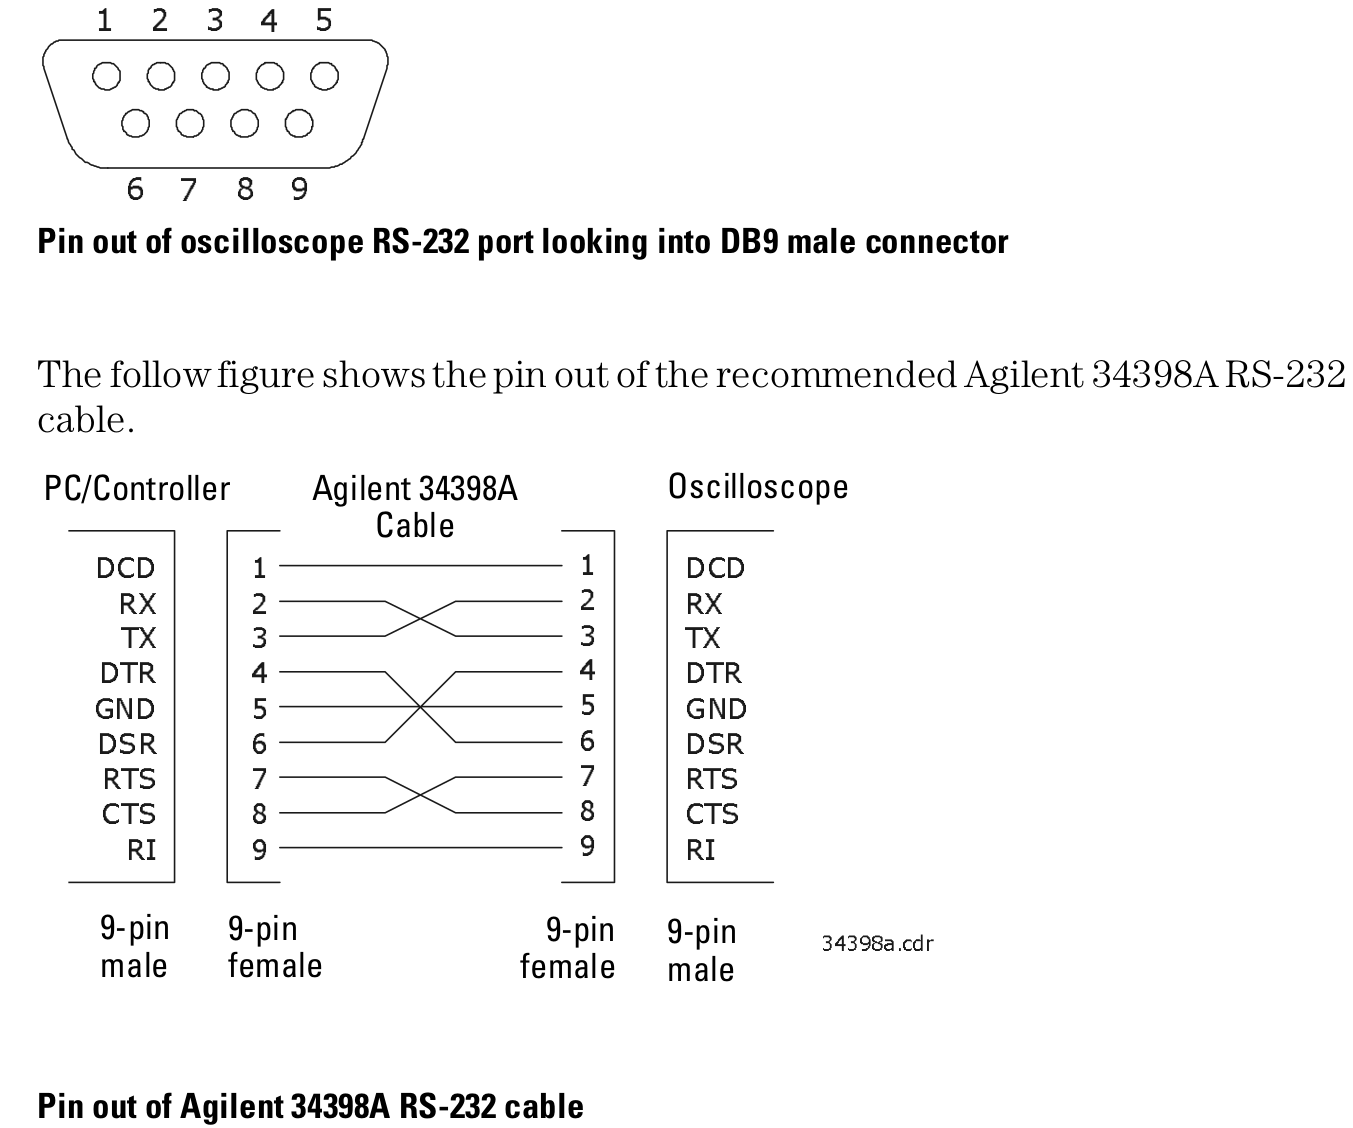
\includegraphics[width=\textwidth]{Agilent-RS232-pinout}
    \caption{%
        Zapojení kabelu pro propojení osciloskopu Agilent~54621A
        s~počítačem~\cite{Agilent54621Auser}
    }
    \label{fig:agilent RS232 pinout}
\end{figure}

Program napsaný v jazyce Python je uložen v souboru \filename{scrot}:
\lstinputlisting[language=Python,style=numbers]{prilohy/scrot}

Po získání nekomprimovaného obrázku ve formátu BMP je vhodné provést
bezztrátovou konverzi do formátu PNG příkazem \shellcmd{convert} z balíčku
\texttt{imagemagick}.
Příklad použití v prostředí operačního systému GNU/Linux:
\begin{lstlisting}[style=terminal]
$ ./scrot -h
usage: scrot [-h] device file

positional arguments:
  device      Serial port the scope is attached to
  file        File to write the output to

optional arguments:
  -h, --help  show this help message and exit

$ ./scrot /dev/ttyUSB1 nazev-souboru
Screen image written to nazev-souboru.bmp
$ convert nazev-souboru.bmp nazev-souboru.png
$
\end{lstlisting}




\clearpage
\newappendix{Koncový zesilovač s TDA2030}
\label{app:TDA2030}
Při testování zvukového výstupu byl použit jednoduchý nízkofrekvenční koncový
zesilovač s integrovaným obvodem TDA2030, který autor této práce sestavil
v roce 2016 v rámci soutěže v radiotechnice. Na následujícím obrázku je
zobrazen osazovací plán jeho desky plošných spojů a seznam součástek. Schéma
zapojení bohužel není dostupné.
V souboru \filename{prilohy/TDA2030-dokumentace.pdf} je vše, co se zachovalo
z dokumentace tohoto výrobku. Autorem návrhu je OK7PV Petr Vild.

\noindent
\includegraphics[page=2, clip, bb=20mm 89mm 175mm 270mm, width=1.0\textwidth]{prilohy/TDA2030-dokumentace.pdf}



\clearpage
\newappendix{Nastavení firmware Grbl CNC frézy}
\label{app:grbl config}
Po připojení na sériový port frézy pomocí terminálového software (zde program
\shellcmd{minicom}) můžeme přečíst veškerou konfiguraci jejího firmware. Význam
jednotlivých nastavení je vysvětlen v tabulce~\vref{tab:grbl config default}.
\begingroup
\catcode`\-=12
\lstinputlisting[style=terminal]{prilohy/grbl-config.txt}
\endgroup

\begin{table}[H]
    \centering
    \caption{%
        Popis jednotlivých nastavení Grbl a výchozí hodnoty (převzato
        z~\cite{Grblconf})
    }
    \label{tab:grbl config default}
    \begin{otherlanguage*}{english}
        \begin{tabular}{ll}
            \toprule
            Settings and sample values  & Description \\
            \midrule
            \verb|$0=10|                & Step pulse, \si{\micro\second} \\
            \verb|$1=25|                & Step idle delay, \si{\milli\second} \\
            \verb|$2=0|                 & Step port invert, mask \\
            \verb|$3=0|                 & Direction port invert, mask \\
            \verb|$4=0|                 & Step enable invert, boolean \\
            \verb|$5=0|                 & Limit pins invert, boolean \\
            \verb|$6=0|                 & Probe pin invert, boolean \\
            \verb|$10=1|                & Status report, mask \\
            \verb|$11=0.010|            & Junction deviation, \si{\milli\meter} \\
            \verb|$12=0.002|            & Arc tolerance, \si{\milli\meter} \\
            \verb|$13=0|                & Report inches, boolean \\
            \verb|$20=0|                & Soft limits, boolean \\
            \verb|$21=0|                & Hard limits, boolean \\
            \verb|$22=1|                & Homing cycle, boolean \\
            \verb|$23=0|                & Homing dir invert, mask \\
            \verb|$24=25.000|           & Homing feed, \si{\milli\meter\per\minute} \\
            \verb|$25=500.000|          & Homing seek, \si{\milli\meter\per\minute} \\
            \verb|$26=250|              & Homing debounce, \si{\milli\second} \\
            \verb|$27=1.000|            & Homing pull-off, \si{\milli\meter} \\
            \verb|$30=1000|             & Max spindle speed, RPM \\
            \verb|$31=0|                & Min spindle speed, RPM \\
            \verb|$32=0|                & Laser mode, boolean \\
            \verb|$100=250.000|         & X steps/mm \\
            \verb|$101=250.000|         & Y steps/mm \\
            \verb|$102=250.000|         & Z steps/mm \\
            \verb|$110=500.000|         & X Max rate, \si{\milli\meter\per\minute} \\
            \verb|$111=500.000|         & Y Max rate, \si{\milli\meter\per\minute} \\
            \verb|$112=500.000|         & Z Max rate, \si{\milli\meter\per\minute} \\
            \verb|$120=10.000|          & X Acceleration, \si{\milli\meter\per\second\squared} \\
            \verb|$121=10.000|          & Y Acceleration, \si{\milli\meter\per\second\squared} \\
            \verb|$122=10.000|          & Z Acceleration, \si{\milli\meter\per\second\squared} \\
            \verb|$130=200.000|         & X Max travel, \si{\milli\meter} \\
            \verb|$131=200.000|         & Y Max travel, \si{\milli\meter} \\
            \verb|$132=200.000|         & Z Max travel, \si{\milli\meter} \\
            \bottomrule
        \end{tabular}
    \end{otherlanguage*}
\end{table}



\clearpage
\newappendix{Skript pro automatickou aktualizaci Home Assistant}
\label{app:update ha}
\lstinputlisting[language=mybash,style=numbers]{prilohy/update_ha}



\clearpage
\includepdf[
    pages=1,
    %landscape,
    angle=90,
    noautoscale,
    width=\linewidth,
    %height=\textheight,
    % trial and error with frame and geometry's showframe, both width and
    % height specified
    offset=12.5mm 2.6mm,
    %frame,
    pagecommand={%
        \newappendix{Schéma zapojení a návrh hlavní DPS}
        \label{app:PCB main}
    },
]{prilohy/AlarmClock-hardware/AlarmClock/AlarmClock.pdf}

\includepdf[
    pages={2-last},
    %landscape,
    angle=90,
    noautoscale,
    width=\linewidth,
    %height=\textheight,
    offset=12.5mm 2.6mm,
    %frame,
    pagecommand={},
]{prilohy/AlarmClock-hardware/AlarmClock/AlarmClock.pdf}

\includepdf[
    pages=-,
    %landscape,
    angle=90,
    noautoscale,
    width=\linewidth,
    %height=\textheight,
    offset=12.5mm 2.6mm,
    %frame,
    pagecommand={},
]{prilohy/AlarmClock-hardware/AlarmClock/AlarmClock-PCB.pdf}

\begin{figure}[htbp]
    \centering
    \subcaptionbox{přední strana}{%
        \includegraphics[height=0.45\textheight]{prilohy/AlarmClock-hardware/AlarmClock/3d/AlarmClock-top.png}
    }
    \subcaptionbox{zadní strana}{%
        \includegraphics[height=0.45\textheight]{prilohy/AlarmClock-hardware/AlarmClock/3d/AlarmClock-bottom.png}
    }
    \caption{3D vizualizace DPS}
    \label{fig:PCB 3d}
\end{figure}



\clearpage
\includepdf[
    pages=1,
    %landscape,
    angle=90,
    noautoscale,
    width=\linewidth,
    %height=\textheight,
    % trial and error with frame and geometry's showframe, both width and
    % height specified
    offset=12.5mm 2.6mm,
    %frame,
    pagecommand={%
        \newappendix{Schéma zapojení a návrh DPS pro otočný enkodér}
        \label{app:PCB encoder}
    },
]{prilohy/AlarmClock-hardware/AlarmClock-encoder/AlarmClock-encoder.pdf}

\includepdf[
    pages=-,
    %landscape,
    angle=90,
    noautoscale,
    width=\linewidth,
    %height=\textheight,
    offset=12.5mm 2.6mm,
    %frame,
    pagecommand={},
]{prilohy/AlarmClock-hardware/AlarmClock-encoder/AlarmClock-encoder-PCB.pdf}




\newappendix{Měření charakteristiky stmívače}
\label{app:ambient}
Průběh závislosti proudu protékajícího výkonovou LED na požadovaném jasu (číslo
v rozsahu \numrange{0}{255}) lze změřit metodou bod po bodu. Digitální
ampérmetr je připojen v sérii s LED, zadaný jas je nastavován přes sériový port
budíku. S digitálním multimetrem Owon B35T, který podporuje připojení
k počítači přes Bluetooth, lze provést měření zcela automaticky s pomocí
následujícího programu:
\lstinputlisting[language=Python,style=numbers]{prilohy/measure_ambient.py}

\begin{lstlisting}[style=terminal]
$ ./measure_ambient.py
duty; value
0;2022-04-10 15:53:14.949140;0.0;mA;(DC-auto)
10;2022-04-10 15:53:24.769441;0.0;mA;(DC-auto)
20;2022-04-10 15:53:35.191933;0.61;mA;(DC-auto)
30;2022-04-10 15:53:45.012132;2.6;mA;(DC-auto)
40;2022-04-10 15:53:55.433162;6.78;mA;(DC-auto)
50;2022-04-10 15:54:05.454056;12.94;mA;(DC-auto)
60;2022-04-10 15:54:15.273836;20.42;mA;(DC-auto)
70;2022-04-10 15:54:25.694675;28.72;mA;(DC-auto)
80;2022-04-10 15:54:35.716312;37.5;mA;(DC-auto)
90;2022-04-10 15:54:45.736972;46.6;mA;(DC-auto)
100;2022-04-10 15:54:55.558120;55.89;mA;(DC-auto)
110;2022-04-10 15:55:05.578489;65.3;mA;(DC-auto)
120;2022-04-10 15:55:15.800582;74.8;mA;(DC-auto)
130;2022-04-10 15:55:26.021199;84.4;mA;(DC-auto)
140;2022-04-10 15:55:35.642069;93.8;mA;(DC-auto)
150;2022-04-10 15:55:45.663607;103.0;mA;(DC-auto)
160;2022-04-10 15:55:56.286673;111.7;mA;(DC-auto)
170;2022-04-10 15:56:06.306743;119.6;mA;(DC-auto)
180;2022-04-10 15:56:15.926708;126.1;mA;(DC-auto)
190;2022-04-10 15:56:26.146637;131.5;mA;(DC-auto)
200;2022-04-10 15:56:36.167047;135.3;mA;(DC-auto)
210;2022-04-10 15:56:46.387852;137.9;mA;(DC-auto)
220;2022-04-10 15:56:56.207813;139.8;mA;(DC-auto)
230;2022-04-10 15:57:06.429305;141.2;mA;(DC-auto)
240;2022-04-10 15:57:16.450719;142.3;mA;(DC-auto)
250;2022-04-10 15:57:26.471619;143.5;mA;(DC-auto)
255;2022-04-10 15:57:36.693283;143.6;mA;(DC-auto)
done
\end{lstlisting}

\noindent
\begin{minipage}[t]{1.00\textwidth}
    \centering
    \captionsetup{type=table}
    \caption{%
        Naměřené hodnoty závislosti velikosti proudu protékajícího výkonovou
        LED na požadovaném jasu stmívače
    }
    \label{tab:hodnoty ambient}
    \CatchFileDef{\tabambient}{hodnoty/c_ambient.tex}{}
    \sisetup{
        table-number-alignment = center
    }
    \begin{tabular}{
            S[table-format=3.0]
            S[table-format=3.2]
        }
        \toprule
        {Požadovaný jas (\numrange{0}{255})}
        & {$I_\mathrm{LED}\,[\si{\milli\ampere}]$}
        \\
        \midrule
        \tabambient
        \bottomrule
    \end{tabular}
\end{minipage}

\clearpage
\begin{landscape}
    \begin{figure}[H]
        \centering
        \input{hodnoty/graf-ambient.tex}
        \caption{%
            Naměřená závislost velikosti proudu protékajícího výkonovou LED na
            požadovaném jasu stmívače
        }
        \label{fig:graf ambient}
    \end{figure}
\end{landscape}


\clearpage
\todo[inline]{cislovani obrazku a tabulek v prilohach}
